
\documentclass{report}

\usepackage[utf8]{inputenc}
\usepackage[italian]{babel}
\usepackage{import}
\usepackage{todonotes}
\usepackage{color}
\usepackage{rotating}
\usepackage[hidelinks]{hyperref}
\usepackage{url}
\usepackage{pdfpages}
\usepackage{siunitx}
\usepackage{pdflscape}
\usepackage{subfig}
\usepackage[euler]{textgreek}
\usepackage{mhchem}

\usepackage{multirow}

\usepackage{enumerate} 
\usepackage{amsmath}
\usepackage{amsfonts}

\usepackage[signatures,swapnames,sans]{frontespizio}

\usepackage{geometry}
\geometry{portrait, margin=3cm}
\usepackage{siunitx}
\usepackage{booktabs}

\renewcommand*\figurename{Figura}

\newcommand{\sub}[1]{\textsubscript{#1}}
\newcommand{\super}[1]{\textsuperscript{#1}}
\newcommand{\parallelsum}{\mathbin{\!/\mkern-5mu/\!}}

\newcommand{\Fig}[0]{Fig.}

\usepackage{titlesec}

\titleformat{\chapter}{\normalfont\huge}{}{20pt}{\huge\bfseries}

\linespread{1.3}


%% COMANDI UTILI
%\begin{table}[h]
%	\centering
%	\begin{tabular}{|c|c|c|}
%	\cline{2-3} 
%	\multicolumn{1}{c|}{} & \textbf{Valore nominale} & \textbf{Valore misurato}\\ 
%		%\hline
%		%{} & \textbf{Valore nominale} & \textbf{Valore misurato} \\ 
%		\hline
%		$\mathbf{R_1}$ & \SI{18}{k\ohm} & \SI{17.977}{k\ohm} \\ 
%		\hline
%		$\mathbf{R_2}$& \SI{1.8}{k\ohm} & \SI{1.815}{k\ohm} \\ 
%		\hline
%	\end{tabular}
%\caption{Misure delle resistenze utilizzate per il circuito.}
%\label{table:mis_res}
%\end{table}
%\begin{figure}[h!]
%\centering
%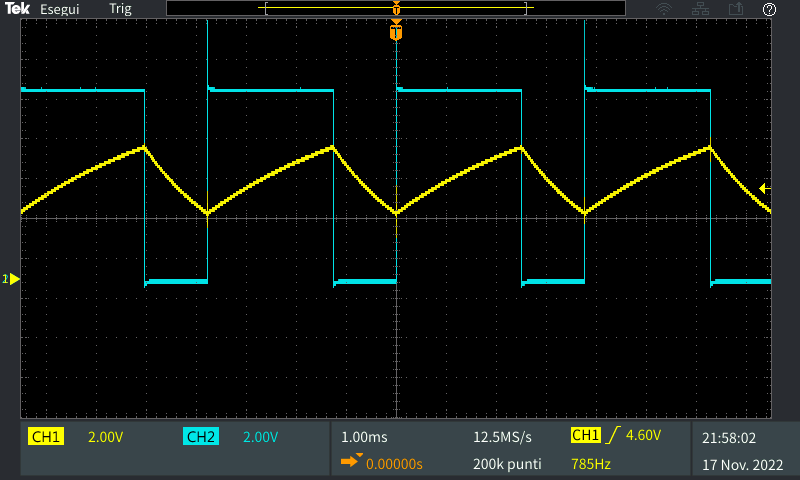
\includegraphics[height=6.5cm]{immagini/TEK00018}\\(a)\\[1ex]
%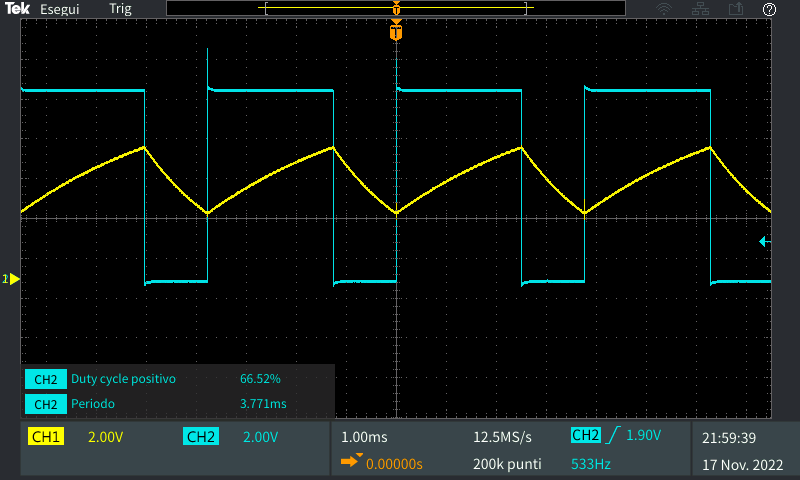
\includegraphics[height=6.5cm]{immagini/TEK00019}\\(b)
%\caption{Risposta del circuito con accoppiamento DC (a) e accoppiamento AC (b).}
%	\label{figura:accopp}
%\end{figure}

\begin{document}
\addtocounter{chapter}{+4}
	\begin{frontespizio}
		\Margini{3cm}{3cm}{3cm}{3cm}
		\Universita{Bergamo}
		\Logo[43.332mm]{unibg-mark}
		\Divisione{Scuola di Ingegneria}
		\Corso[Laurea Magistrale]{Ingegneria Informatica}
		\Titolo{Laboratorio di Elettronica}
		\Sottotitolo{Relazione esperienza di laboratorio 5}
		\Punteggiatura{}
		\NRelatore{Prof.}{Prof.}
		\Relatore{Luigi Gaioni}
		\Candidato[1058231]{Giulia Allievi}
		\Candidato[1059640]{Martina Fanton}
		\Annoaccademico{2022--2023}
		\begin{Preambolo*}
			\usepackage[italian]{babel}
			\usepackage[T1]{fontenc}
			\usepackage[utf8]{inputenc}
			\usepackage{microtype}
			\usepackage{lmodern}
			\graphicspath{{img/}}
			
			\renewcommand{\frontinstitutionfont}{\fontsize{14}{17}\bfseries\scshape}
			\renewcommand{\fronttitlefont}{\fontsize{17}{21}\bfseries\scshape}
			\renewcommand{\frontfootfont}{\fontsize{12}{14}\bfseries\scshape}
		\end{Preambolo*}
	\end{frontespizio}

%----------------------------------------------------------------------------------------
%	PAGINA BIANCA
%----------------------------------------------------------------------------------------
\newpage
\null
\thispagestyle{empty}
\newpage

%----------------------------------------------------------------------------------------
%	INTRO
%----------------------------------------------------------------------------------------
\chapter{Relazione attività di laboratorio 5}
\section*{Introduzione}
In quest'attività di laboratorio abbiamo visto un ultimo circuito monostabile con NE555, successivamente sono state analizzate le altre due configurazioni realizzabili con questo circuito integrato (prima la configurazione bistabile e dopo quella astabile).  \par
La seconda modalità, quella astabile, permette di generare in uscita al pin 3 un'onda quadra le cui caratteristiche dipendono dalla rete collegata all'esterno del circuito integrato. Le connessioni sono illustrate nel datasheet del componente, si riporta di seguito lo schema (figura \ref{figura:datasheet1}).
\begin{figure}[h!]
	\centering
	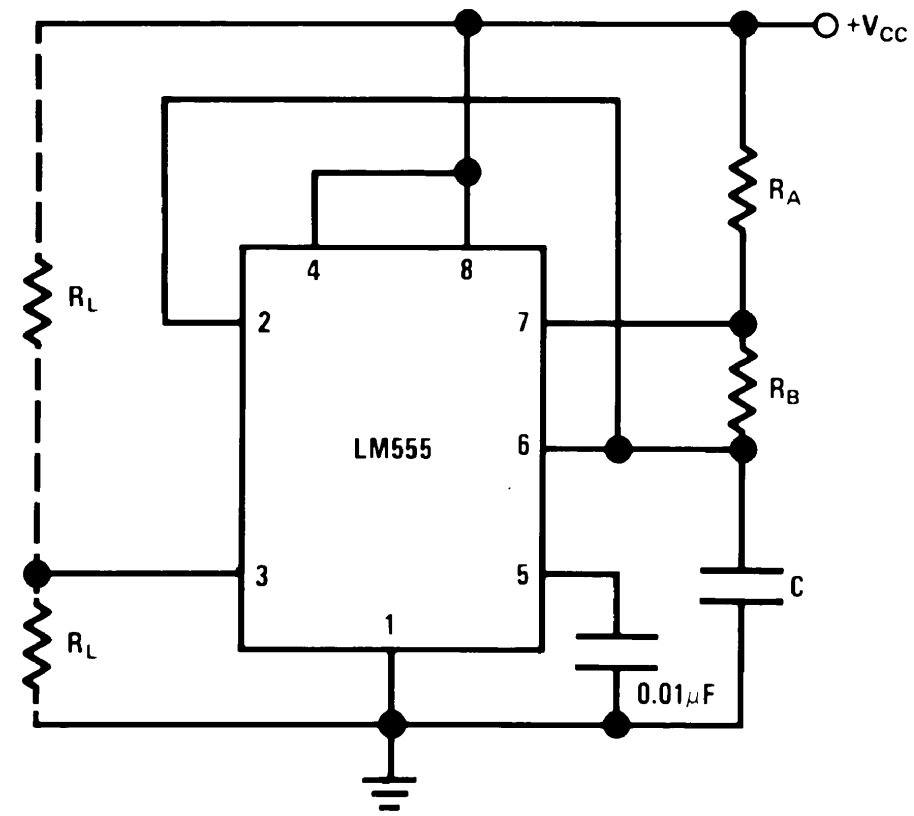
\includegraphics[height=6cm]{immagini/datasheet1}
	\caption{Schema delle connessioni da utilizzare per ottenere un circuito astabile (fonte: \textcolor{blue}{\underline{\href{https://www.ti.com/lit/ds/symlink/lm555.pdf?ts=1667144089940&ref_url=https\%253A\%252F\%252Fwww.ti.com\%252Fproduct\%252FLM555}{datasheet}}}).} % LM o NE ??
	\label{figura:datasheet1}
\end{figure}
\\ La configurazione bistabile invece non è presentata nel datasheet. Questa modalità è utile quando si vuole utilizzare il NE555 come flip-flop set reset. Per ottenerla, è sufficiente utilizzare due resistenze e due pulsanti. Una resistenza è collegata tra i pin 8 e 2, l'altra invece è collegata tra i pin 4 e 8; per quanto riguarda i due pulsanti, uno è collegato tra i pin 2 e 1 e pilota il set, mentre l'altro è connesso ai pin 4 e 1 e comanda il reset. Il pin 8 è collegato all'alimentazione, il pin 1 a massa, il segnale è prelevato al pin 3 e tutti gli altri pin sono lasciati floating. Lo schema si trova nella sezione dedicata all'analisi di questo circuito (sezione \ref{sez2}, figura \ref{figura:schema2}).

\newpage
\section{Circuito 1: NE555 in configurazione monostabile con switch debouncing}
\subsection{Schema del circuito e Funzione di Trasferimento}
Questo circuito è basato sul circuito monostabile con NE555 (analizzato nello scorso laboratorio). La differenza più evidente tra i due circuiti è rappresentata dal fatto che il circuito in esame riceve in ingresso un segnale di trigger generato da un pulsante, mentre il precedente circuito riceveva in ingresso un segnale di trigger fornito da un generatore di forme d'onda.

Questo circuito, mostrato in figura \ref{figura:schema1}, presenta: due resistenze (R è collegata tra il pin 7 e l'alimentazione positiva, mentre $\mathrm{R_1}$ tra il pin 2 e l'alimentazione positiva), due capacità ($\mathrm{C_1}$ è collegata tra il pin 6 e la massa, mentre $\mathrm{C_2}$ tra il pin 5 e la massa) e un pulsante collegato tra il pin 2 e la massa. I pin 6 e 7 sono cortocircuitati.

\begin{figure}[h!]
	\centering
	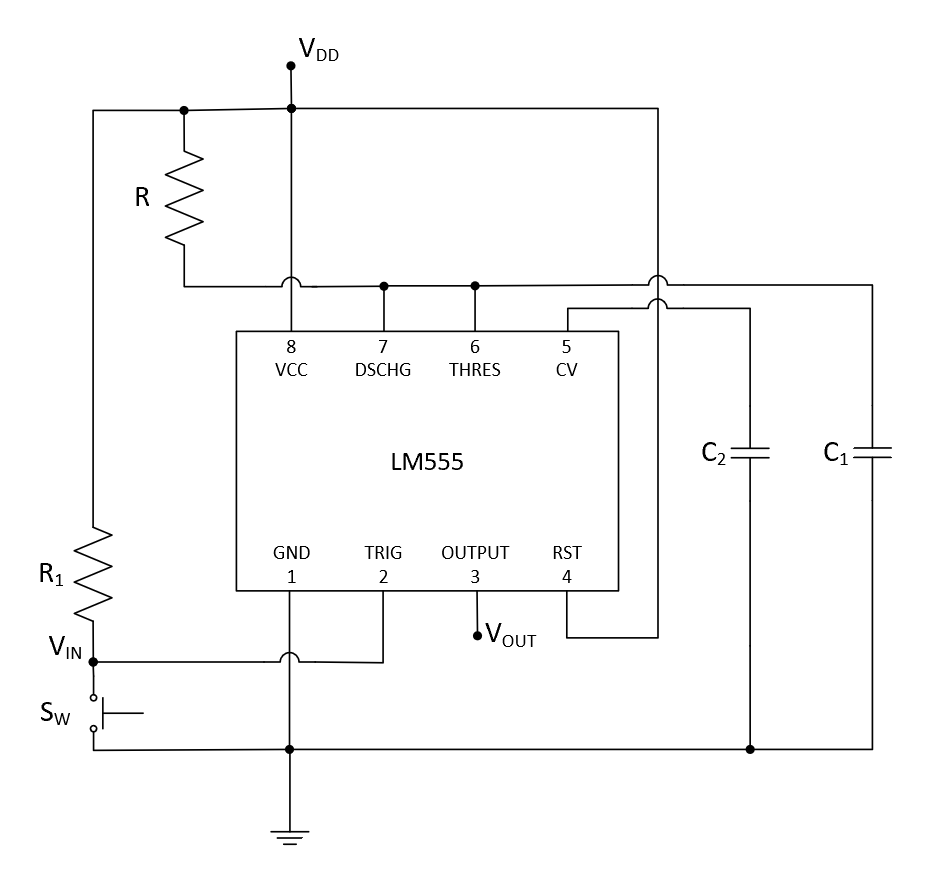
\includegraphics[height=6.5cm]{immagini/schema1}
	\caption{Schema del circuito monostabile con switch debouncing.}
	\label{figura:schema1}
\end{figure}

\noindent La caratteristica principale di questo circuito consiste nel correggere l'effetto del rimbalzo dell'interruttore (\textit{switch debouncing}, visibile nella figura \ref{figura:TEK00009}). Questo effetto, che consiste nella generazione di un treno di impulsi spuri su entrambi i fronti dell'impulso in ingresso, viene prodotto dalla rete antecedente il timer e in particolare è dovuto al fatto che la chiusura e l'apertura del pulsante non avvengono in modo istantaneo, perché c'è un transitorio dovuto ai componenti meccanici dell'interruttore. L'aggiunta del NE555 alla rete in ingresso (e in particolare a valle dell'interruttore) determina un segnale in uscita filtrato da questo effetto indesiderato poichè il timer genera un solo impulso in uscita non appena riceve il primo fronte di discesa del segnale in ingresso. % metterei aggiunta 555 a valle dell'interruttore

La funzione di trasferimento di questo circuito è:
\begin{equation}
	\begin{cases}
		V_{out}= V_{DD}\indent\indent \mathrm{a\;partire\;dalla\;chiusura\;di\;} S_W \mathrm{\;e\;per\;una\;durata\;T\;}\\[5pt]
		V_{out}= 0\indent\indent\indent \mathrm{altrimenti}\\
	\end{cases}
\end{equation}

\subsection{Analisi e dati sperimentali}
Per quanto riguarda la scelta e il dimensionamento dei componenti di questo circuito (in figura \ref{figura:circuito1}), come timer è stato scelto un LM555, mentre le due resistenze hanno un valore di \SI{12}{\kilo\ohm}, la capacità $\mathrm{C_1}$ di \SI{10}{\micro\farad} e la capacità $\mathrm{C_2}$ di \SI{1}{\nano\farad}.

\begin{figure}[h!]
	\centering
	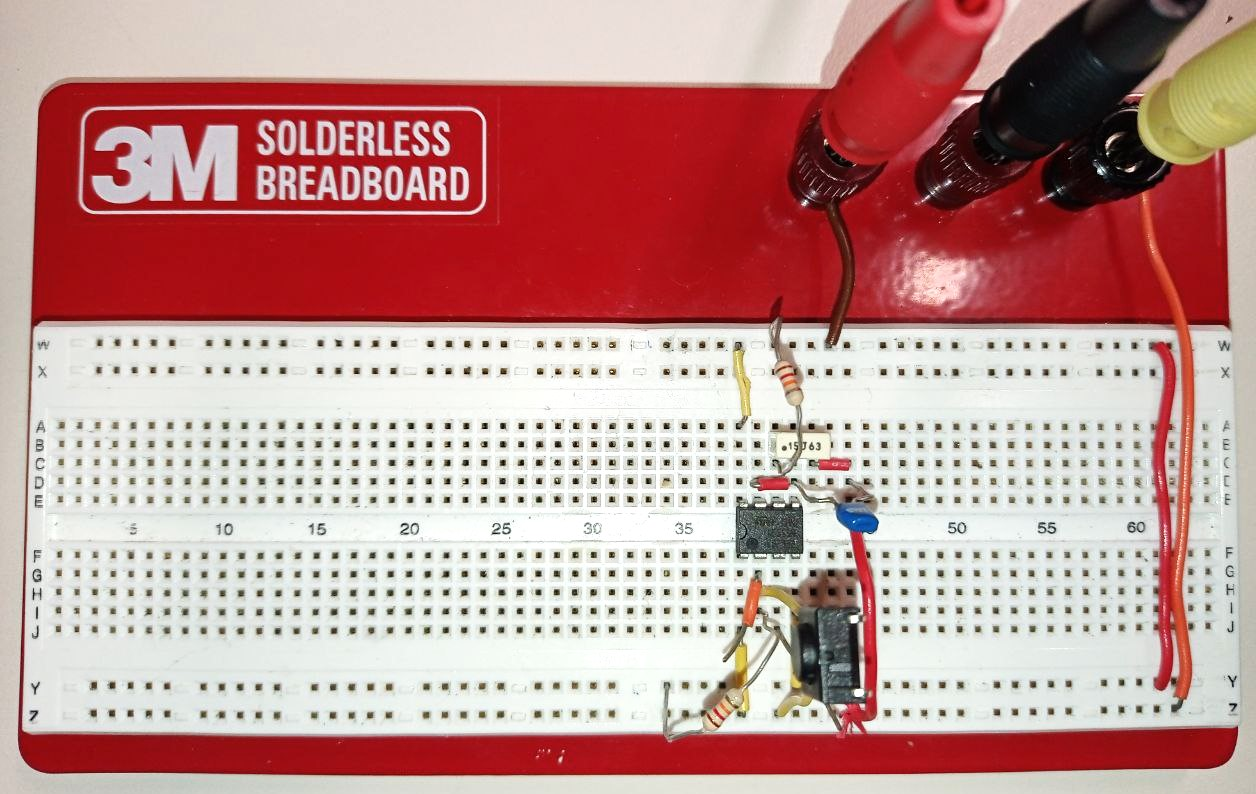
\includegraphics[height=6.8cm]{immagini/circuito1}
	\caption{Fotografia del circuito monostabile con switch debouncing realizzato in laboratorio.}
	\label{figura:circuito1}
\end{figure}

\noindent Avendo dimensionato in questo modo i componenti, ci si aspetta che la durata dell'impulso in uscita al circuito risulti pari a: 
\\\indent$\displaystyle{T = 1.1 \cdot R \cdot C_1 = 1.1 \cdot \SI{12}{\kilo\ohm} \cdot \SI{10}{\micro\farad} = \SI{132}{\milli\second}}$

\noindent Dalla figura \ref{figura:TEK00010} è stato verificato che questa durata assumesse un valore maggiore rispetto alla durata dell'impulso in ingresso (che dalla misura effettuata con i cursori dell'oscilloscopio risulta pari a \SI{120}{\milli\second}).

\begin{figure}[h!]
	\centering
	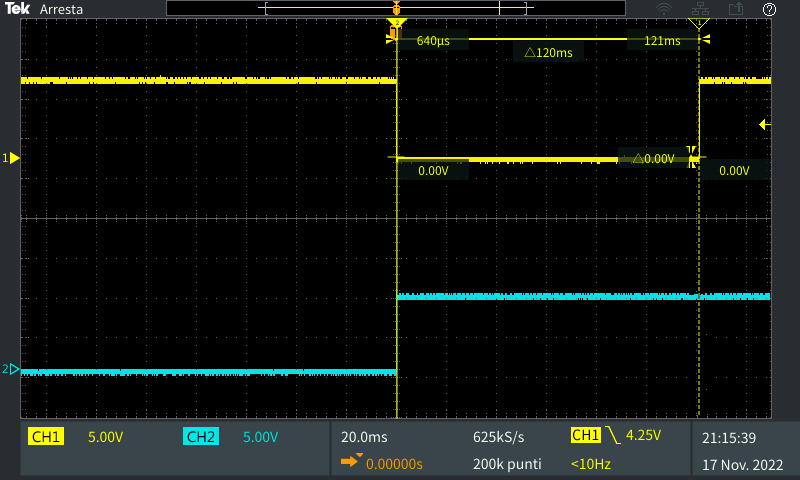
\includegraphics[height=6.3cm]{immagini/TEK00010}
	\caption{Risposta del circuito con cursori.}
	\label{figura:TEK00010}
\end{figure}

\noindent Inoltre dalla figura \ref{figura:TEK00009}, ottenuta ingrandendo l'immagine precedente, si vede che il segnale in uscita al LM555 presenta un solo impulso positivo e di conseguenza il timer ha effettivamente corretto il rimbalzo dell'interruttore, di cui è caratterizzato il segnale in ingresso, come preannunciato nella sezione precedente.

\begin{figure}[h!]
	\centering
	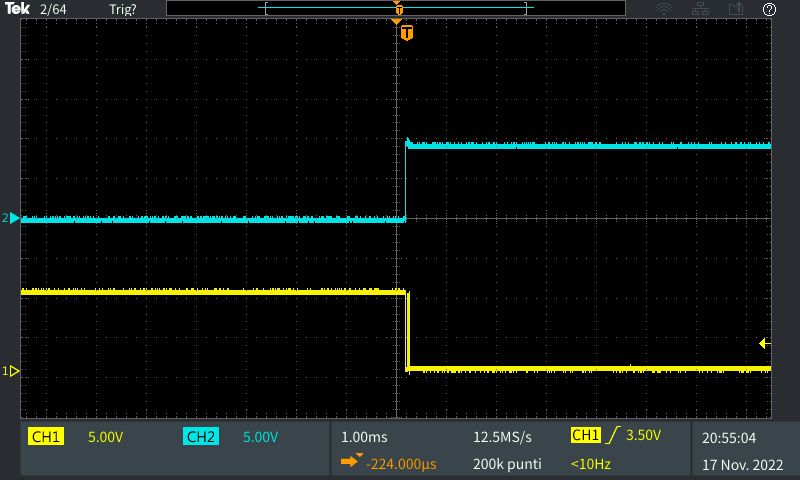
\includegraphics[height=6.5cm]{immagini/TEK00009}
	\caption{Ingrandimento della risposta del circuito (ingresso CH1 e uscita CH2).}
	\label{figura:TEK00009}
\end{figure}

\noindent I grafici delle figure precedenti sono stati ottenuti utilizzando la modalità \textit{Single} dell'oscilloscopio, che permette di visualizzare a schermo segnali costituiti da un impulso definito tramite un pulsante (e quindi segnali non periodici), come il segnale di trigger di questo circuito. Anche per i prossimi circuiti analizzati servirà utilizzare questa modalità dell'oscilloscopio.

\newpage
\section{Circuito 2: LM555 in configurazione bistabile}\label{sez2}
\subsection{Schema del circuito e Funzione di Trasferimento}
Questo circuito (in figura \ref{figura:schema2}) è costituito da un timer NE555, da due resistenze (dette resistenze di pull-up) e da due pulsanti (uno per il set e uno per il reset).

\begin{figure}[h!]
	\centering
	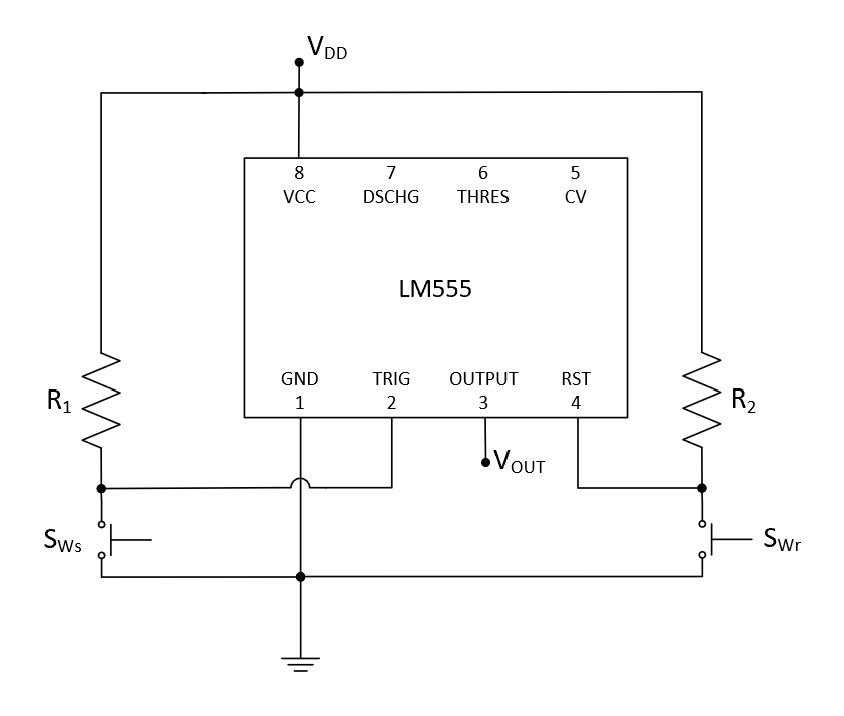
\includegraphics[height=8cm]{immagini/schema2}
	\caption{Schema del circuito bistabile.}
	\label{figura:schema2}
\end{figure}

\noindent Si tratta di un circuito bistabile perché presenta due stati stabili, set e reset, che vengono attivati in modo mutuamente esclusivo tramite la pressione alternata di due pulsanti situati tra i rispettivi nodi e la massa.

Dunque in ingresso si riceve un segnale che può essere di due tipologie differenti in base all'interruttore premuto: uno per il set oppure uno per il reset che determinano in uscita una transizione al livello logico alto o a quello basso rispettivamente.

Perciò la durata dell'impulso positivo presente sul segnale in uscita dipende dal momento in cui il NE555 riceve ciascuno dei due comandi. In particolare il momento della ricezione del comando di set determina l'istante del fronte di salita dell'impulso, mentre la ricezione del comando di reset ne determina l'istante del fronte di discesa.

La funzione di trasferimento di questo circuito è:
\begin{equation}
	\begin{cases}
		V_{out}= V_{DD}\indent\indent \mathrm{a\;partire\;dalla\;pressione\;di\;} S_{Ws} \mathrm{\;fino\;alla\;pressione\;di\;} S_{Wr}\\[5pt]
		V_{out}= 0\indent\indent\indent \mathrm{a\;partire\;dalla\;pressione\;di\;} S_{Wr} \mathrm{\;fino\;alla\;pressione\;di\;} S_{Ws}\\ % MOD
	\end{cases}
\end{equation}

\subsection{Analisi e dati sperimentali}
Per realizzare il circuito (visibile in figura \ref{figura:circuito2}) sono state utilizzate due resistenze con un valore di \SI{10}{\kilo\ohm} ciascuna.

\begin{figure}[h!]
	\centering
	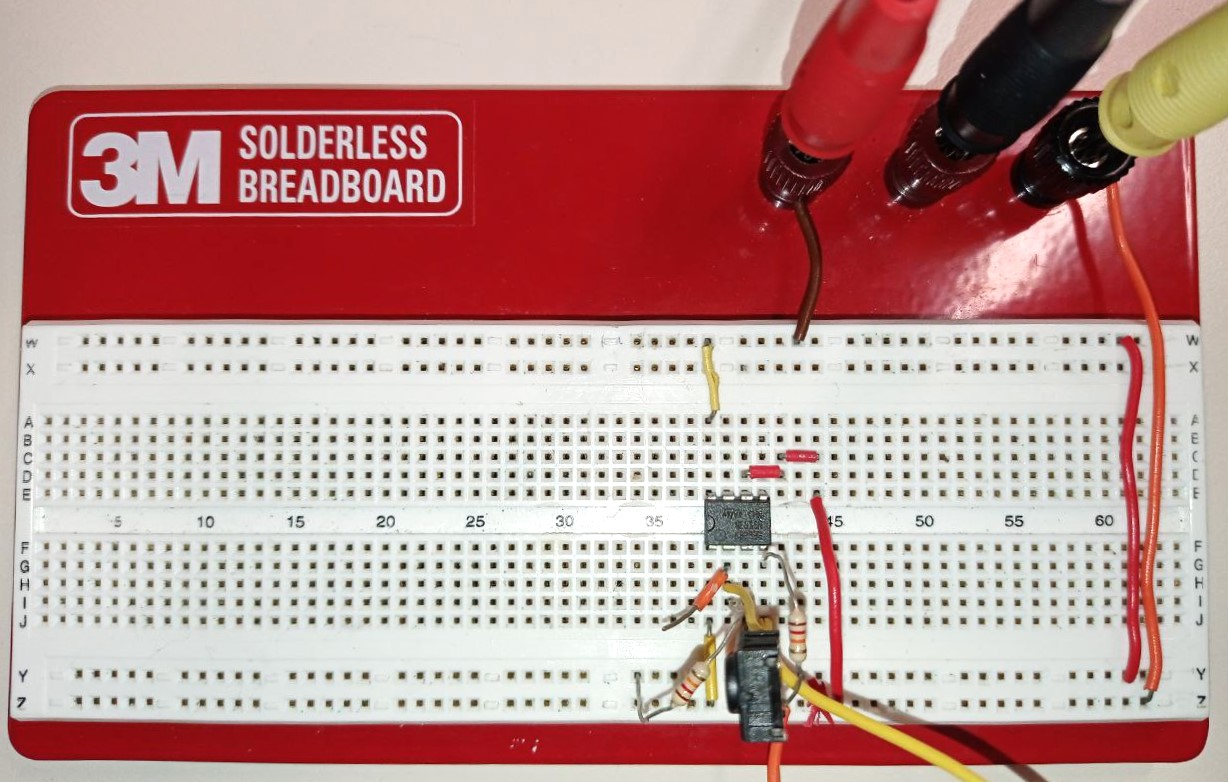
\includegraphics[height=7cm]{immagini/circuito2}
	\caption{Fotografia del circuito bistabile realizzato in laboratorio.}
	\label{figura:circuito2}
\end{figure}

\noindent Inizialmente è stato premuto il pulsante di set (mantenendo il pulsante di reset aperto) e questo ha consentito di avere in uscita un segnale al livello logico alto, perciò si entra nello stato stabile di set.

Successivamente è stato premuto il pulsante di reset (mantenendo il pulsante di set aperto), ottenendo di conseguenza in uscita un segnale al livello logico basso, quindi si passa dallo stato stabile di set a quello stabile di reset.

Queste variazioni sull'uscita sono state riportate nella figura \ref{figura:TEK00012e13} in cui sono rappresentati in giallo l'ingresso (a sinistra il set e a destra il reset) e in azzurro l'uscita.

\begin{figure}[h!]
	\centering
	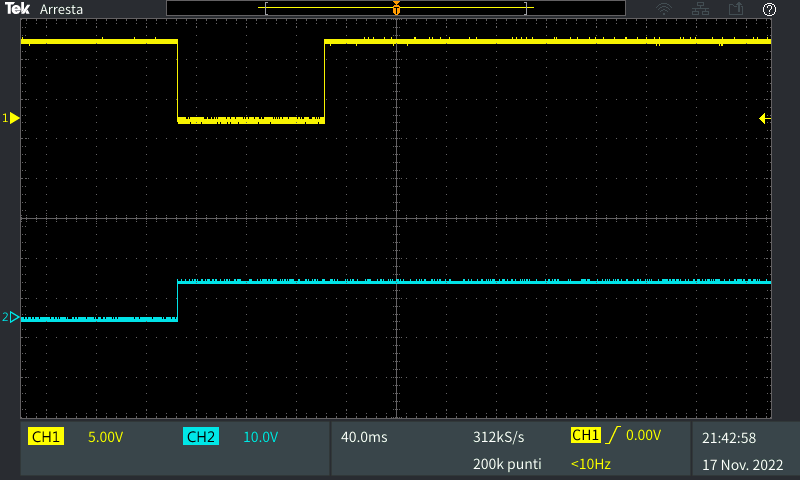
\includegraphics[height=4.6cm]{immagini/TEK00016}
	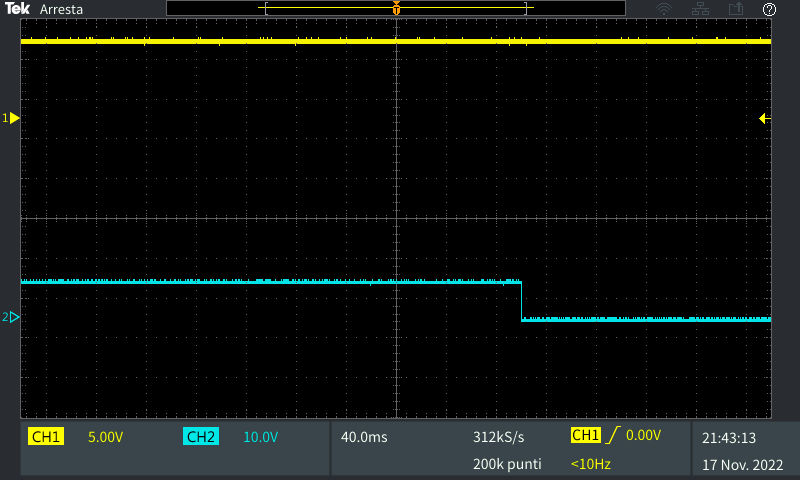
\includegraphics[height=4.6cm]{immagini/TEK00017}
	\caption{Risposta del circuito: a sinistra S ON - R OFF, a destra S OFF - R ON.}
	\label{figura:TEK00012e13}
\end{figure}

\newpage
\section{Circuito 3: LM555 in configurazione astabile}
\subsection{Schema del circuito e Funzione di Trasferimento}
Andiamo ora a studiare l'ultima configurazione del NE555, che è la modalità astabile. Per realizzare il circuito, si utilizzano due capacità e due resistenze: la prima resistenza, $\mathrm{R_A}$, è collegata fra l'alimentazione e il pin 7 del NE555, mentre la seconda, $\mathrm{R_B}$, si trova fra i pin 7 e 2; per quanto riguarda le capacità, $\mathrm{C_1}$ si trova tra il pin 6 e la massa, invece $\mathrm{C_2}$ è connessa tra il pin 5 e la massa. Lo schema si trova in figura \ref{figura:schema3}. \par
In quest'ultima configurazione, il NE555 viene utilizzato per generare un'onda quadra con duty cycle variabile, le cui caratteristiche dipendono dalla rete collegata esternamente al componente. Non abbiamo nessuno stato stabile, l'uscita oscillerà continuamente tra due stati instabili.
\begin{figure}[h!]
	\centering
	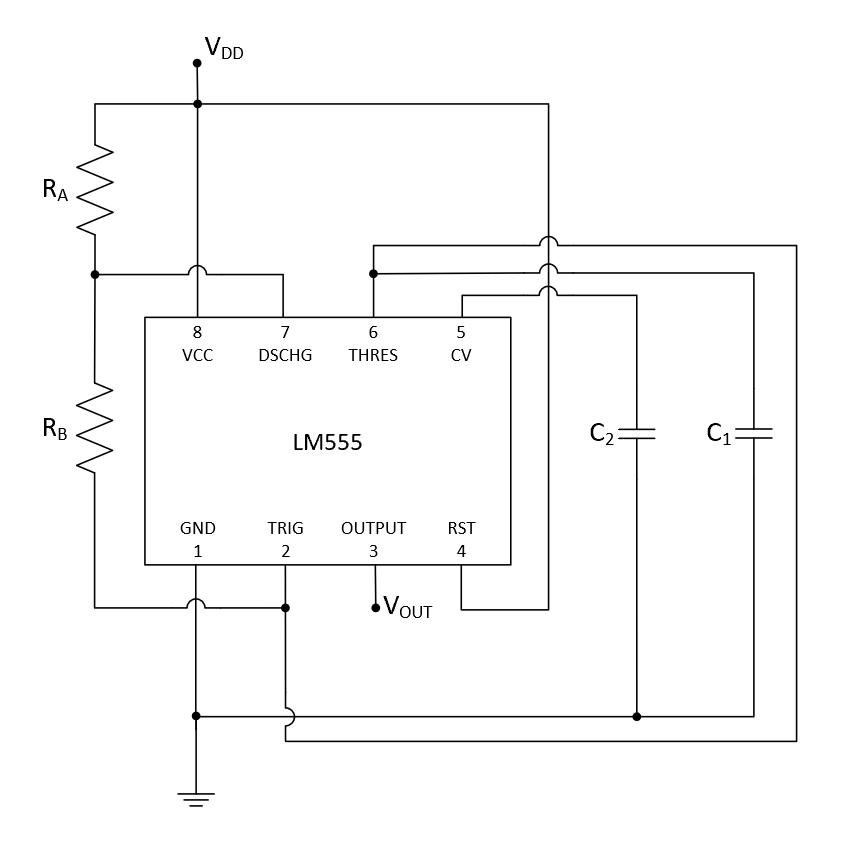
\includegraphics[height=8cm]{immagini/schema3}
	\caption{Schema del circuito astabile.}
	\label{figura:schema3}
\end{figure}
\\Il percorso di carica della capacità $\mathrm{C_1}$ avviene attraverso la serie delle resistenze $\mathrm{R_A}$ e $\mathrm{R_B}$: la fase di carica ha inizio quando la tensione ai capi della capacità è di $1/3\cdot V_{DD}$ e termina quando questo valore raggiunge $2/3\cdot V_{DD}$. Durante quest'intervallo di tempo, $t_1$, l'uscita va a $\mathrm{V_{DD}}$, quindi rimane alta. Terminata la fase di carica, ha inizio la fase di scarica della capacità $\mathrm{C_1}$ attraverso la resistenza $\mathrm{R_B}$. La scarica continua fin quando la tensione ai capi di $\mathrm{C_1}$ raggiunge il valore di $1/3\cdot V_{DD}$ e durante questo periodo di tempo, $t_2$, l'uscita va a massa, dunque rimane bassa. 
\\Le fasi di carica e scarica si alternano continuamente nel tempo, la loro durata si calcola come segue:
\\[4pt]\indent$\displaystyle{t_1 = (R_A+R_B)\cdot C_1\cdot \ln2}$
\\[4pt]\indent$\displaystyle{t_2 = R_B\cdot C_1\cdot \ln2}$
\\[4pt]\indent$\displaystyle{\rightarrow T=t_1+t_2\indent\Rightarrow f=\frac{1}{t_1+t_2}}$
\\[4pt]Noti $t_1$ e $T$, possiamo calcolare il duty cycle dell'onda quadra, $\delta$:
\\[4pt]\indent$\displaystyle{\delta=\frac{t_1}{T}=\frac{R_A+R_B}{R_A+2\cdot R_B}}$
\\[8pt] Da questa formula, possiamo dire che:
\begin{itemize}
\item se $\displaystyle{R_A\ll R_B\Rightarrow\delta\simeq 50\%}$
\item se $\displaystyle{R_A\gg R_B\Rightarrow\delta\simeq 100\%}$
\end{itemize}
di conseguenza, non sarà possibile ottenere un'onda quadra con duty cycle inferiore al 50\%.
\subsection{Analisi e dati sperimentali}
In figura \ref{figura:circuito3} è riportata la fotografia del circuito realizzato, con $\mathrm{R_A=R_B}$=\SI{12}{k\ohm} e $\mathrm{C_1}$ pari a \SI{150}{n\farad}.
\begin{figure}[h!]
	\centering
	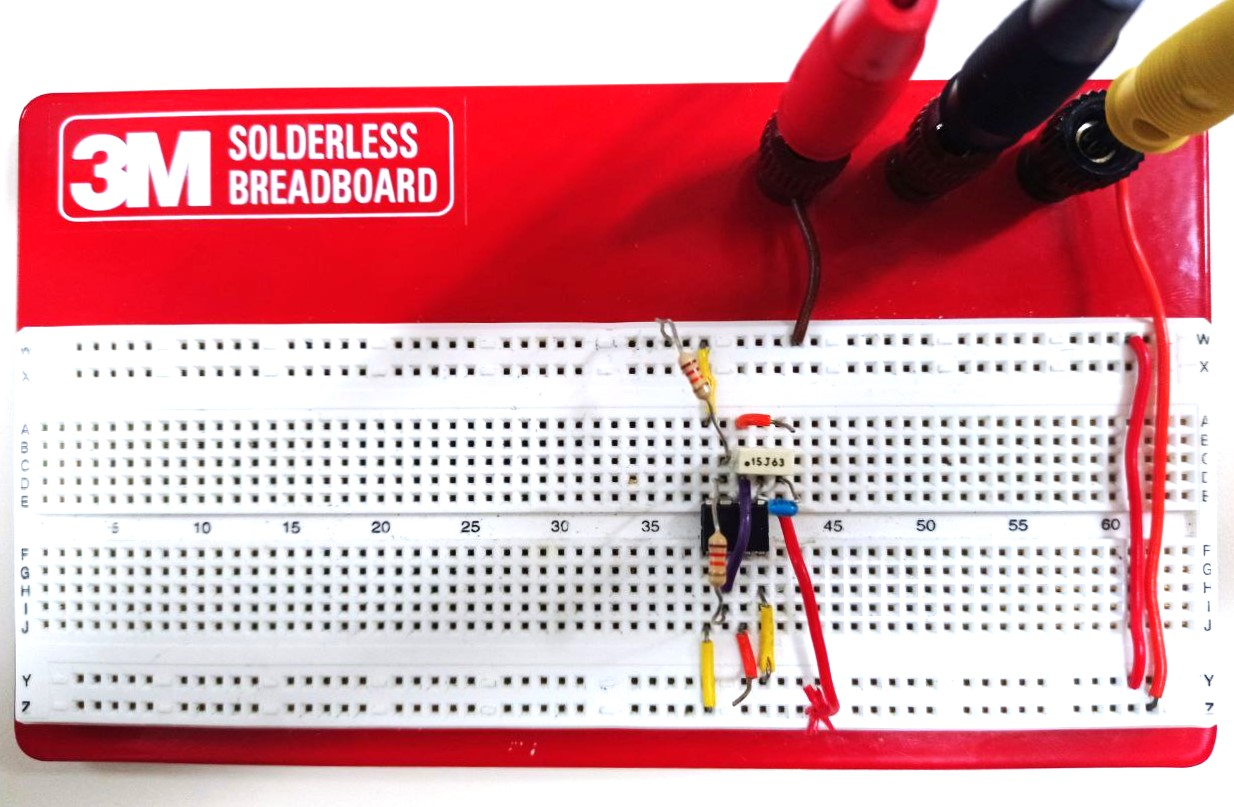
\includegraphics[height=8cm]{immagini/circuito3}
	\caption{Fotografia del circuito astabile realizzato in laboratorio.}
	\label{figura:circuito3}
\end{figure}
\\Il nostro obiettivo è andare a studiare come si comporta il circuito al variare della resistenza $\mathrm{R_A}$ e della capacità $\mathrm{C_1}$. Fissiamo la resistenza $\mathrm{R_B}$ a \SI{12}{k\ohm} e la capacità $\mathrm{C_1}$ a \SI{150}{n\farad}, mentre $\mathrm{R_A}$ varia, i valori utilizzati sono riportati in tabella \ref{table:mis_res3}. Con l'oscilloscopio, andiamo a misurare il periodo e il duty cyle, le misure sono riportate in tabella \ref{table:mis_cto3_1}. \par
Una volta ottenute queste misure, sostituiamo la capacità $\mathrm{C_1}$ con una di valore \SI{68}{n\farad} e ripetiamo le misure, di cui si riportano i risultati in tabella \ref{table:mis_cto3_2}. \par
Successivamente, rielaboriamo tutti questi dati per ottenere dei grafici, dai quali è più immediato capire le caratteristiche del circuito. 
\begin{table}[h!]
	\centering
	\begin{tabular}{|c|c|}
	\hline
		\textbf{Valore nominale} & \textbf{Valore misurato}\\ 
		\hline
		\SI{12}{k\ohm} & \SI{11.973}{k\ohm} \\ 
		\hline
		 \SI{24}{k\ohm} & \SI{23.943}{k\ohm} \\ 
		\hline
		\SI{39}{k\ohm} & \SI{37.621}{k\ohm} \\ 
		\hline
		 \SI{54}{k\ohm} & \SI{54.735}{k\ohm} \\ 
		\hline
		 \SI{82}{k\ohm} & \SI{82.132}{k\ohm} \\ 
		\hline
		 \SI{136}{k\ohm} & \SI{136.867}{k\ohm} \\ 
		\hline
	\end{tabular}
	\caption{Misure delle resistenze utilizzate per il circuito monostabile con LM555.}
	\label{table:mis_res3}
\end{table}
\begin{table}[h!]
	\centering
	\begin{tabular}{|c|c|c|c|c|}
		\hline
		$\mathbf{R_A}$ & \textbf{T teorico} & \textbf{T misurato} & $\mathbf\delta$\textbf{ teorico} & $\mathbf\delta$\textbf{ misurato}\\ 
		\hline
		\SI{12}{k\ohm} & \SI{3.743}{m\second} & \SI{3.771}{m\second} & 66.67\% & 66.52\% \\ 
		\hline
		\SI{24}{k\ohm} & \SI{4.991}{m\second} & \SI{5.048}{m\second} & 75.00\% & 74.94\% \\ 
		\hline
		\SI{39}{k\ohm} & \SI{6.550}{m\second} & \SI{6.502}{m\second} & 80.95\% & 80.54\% \\ 
		\hline
		\SI{54}{k\ohm} & \SI{8.110}{m\second} & \SI{8.325}{m\second} & 84.62\% & 84.77\% \\ 
		\hline
		\SI{82}{k\ohm} & \SI{11.021}{m\second} & \SI{11.250}{m\second} & 88.68\% & 88.71\% \\ 
		\hline
		\SI{136}{k\ohm} & \SI{16.636}{m\second} & \SI{17.180}{m\second} &  92.50\% & 92.61\% \\ 
		\hline
	\end{tabular}
	\caption{Misure e valori teorici con $\mathrm{C_1}$=\SI{150}{n\farad} e $\mathrm{R_B}$=\SI{12}{k\ohm}.}
	\label{table:mis_cto3_1}
\end{table}
\begin{table}[h!]
	\centering
	\begin{tabular}{|c|c|c|c|c|}
		\hline
		$\mathbf{R_A}$ & \textbf{T teorico} & \textbf{T misurato} & $\mathbf\delta$\textbf{ teorico} & $\mathbf\delta$\textbf{ misurato}\\ 
		\hline
		\SI{12}{k\ohm} & \SI{1.697}{m\second} & \SI{1.710}{m\second} & 66.67\% & 66.46\% \\ 
		\hline
		\SI{24}{k\ohm} & \SI{2.262}{m\second} & \SI{2.277}{m\second} & 75.00\% & 74.95\% \\ 
		\hline
		\SI{39}{k\ohm} & \SI{2.969}{m\second} & \SI{2.926}{m\second} & 80.95\% & 80.48\% \\ 
		\hline
		\SI{54}{k\ohm} & \SI{3.677}{m\second} & \SI{3.743}{m\second} & 84.62\% & 84.90\% \\ 
		\hline
		\SI{82}{k\ohm} & \SI{4.996}{m\second} & \SI{5.069}{m\second} & 88.68\% & 88.73\% \\ 
		\hline
		\SI{136}{k\ohm} & \SI{7.541}{m\second} & \SI{7.762}{m\second} & 92.50\% & 92.60\% \\ 
		\hline
	\end{tabular}
	\caption{Misure e valori teorici con $\mathrm{C_1}$=\SI{68}{n\farad} e $\mathrm{R_B}$=\SI{12}{k\ohm}.}
	\label{table:mis_cto3_2}
\end{table}
\newpage
Dalle due tabelle, vediamo che i risultati sperimentali coincidono con quelli teorici per entrambi i valori di capacità. Di seguito, vediamo i grafici in cui si confrontano: il periodo e il duty cycle (misurati e calcolati) della prima capacità usata (figura \ref{figura:graficiC1}), il periodo e il duty cycle (misurati e calcolati) con il secondo valore di capacità (figura \ref{figura:graficiC2}), infine i valori misurati con i due valori (figura \ref{figura:graficiC12}).\par 
Dai grafici delle prime due figure, possiamo confermare che i risultati ottenuti attraverso le misure sono paragonabili a quelli che vengono calcolati con le formule illustrate in precedenza. \par
Dall'ultima figura, invece, possiamo vedere che la relazione che lega $\mathrm{R_A}$ e T è di diretta proporzionalità, infatti all'aumentare del valore della resistenza, aumenta anche T (grafico a sinistra). Anche fra $\mathrm{C_1}$ e T c'è una relazione di proporzionalità, perché all'aumentare della capacità aumenta il periodo T. Per quanto riguarda il duty cycle, questo è inversamente proporzionale alla resistenza $\mathrm{R_A}$, infatti il grafico che otteniamo è un ramo di iperbole (grafico di destra).
\begin{figure}[h!]
	\centering
	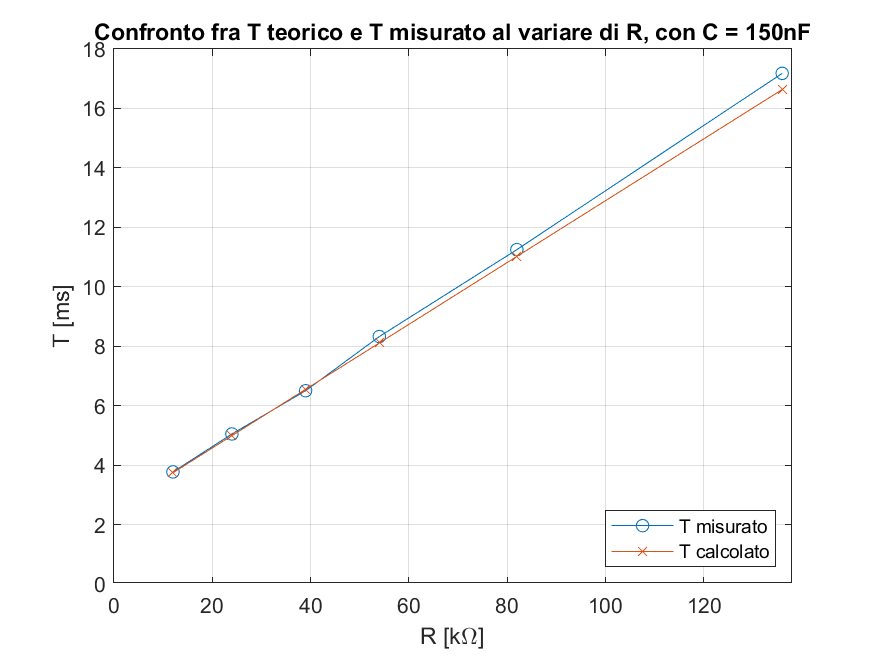
\includegraphics[height=5.8cm]{immagini/graficoT1}
	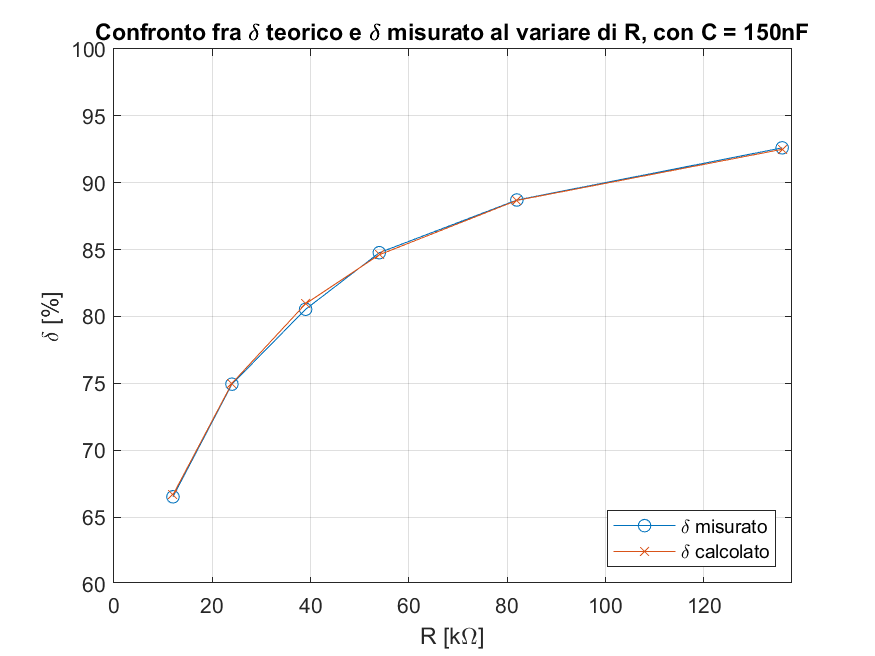
\includegraphics[height=5.8cm]{immagini/graficoDC1}
	\caption{Grafico di T (a sinistra) e $\delta$ (a destra) in funzione di $\mathrm{R_A}$ per $\mathrm{C_1}$ = \SI{150}{n\farad}.}
	\label{figura:graficiC1}
\end{figure}
\begin{figure}[h!]
	\centering
	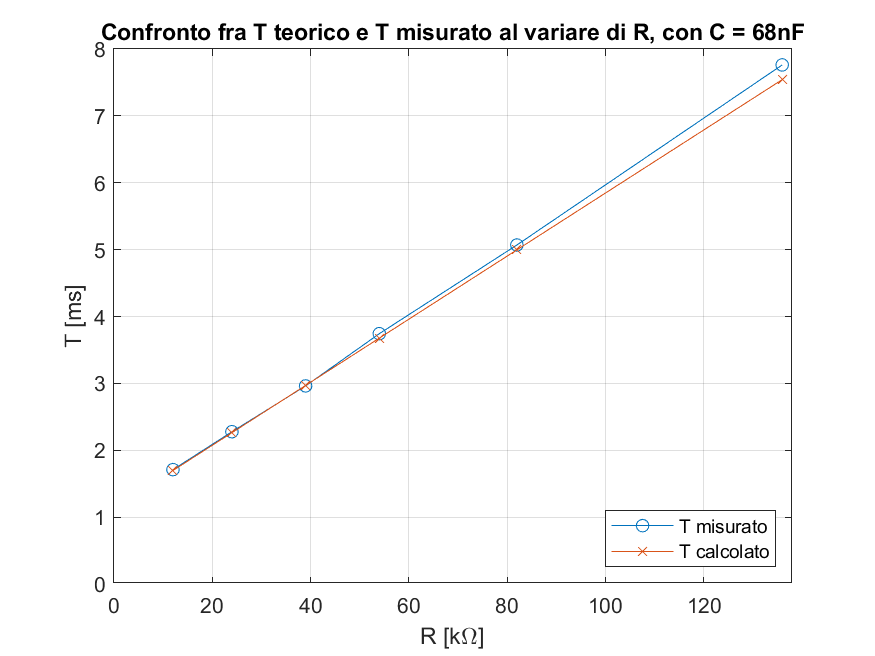
\includegraphics[height=5.8cm]{immagini/graficoT2}
	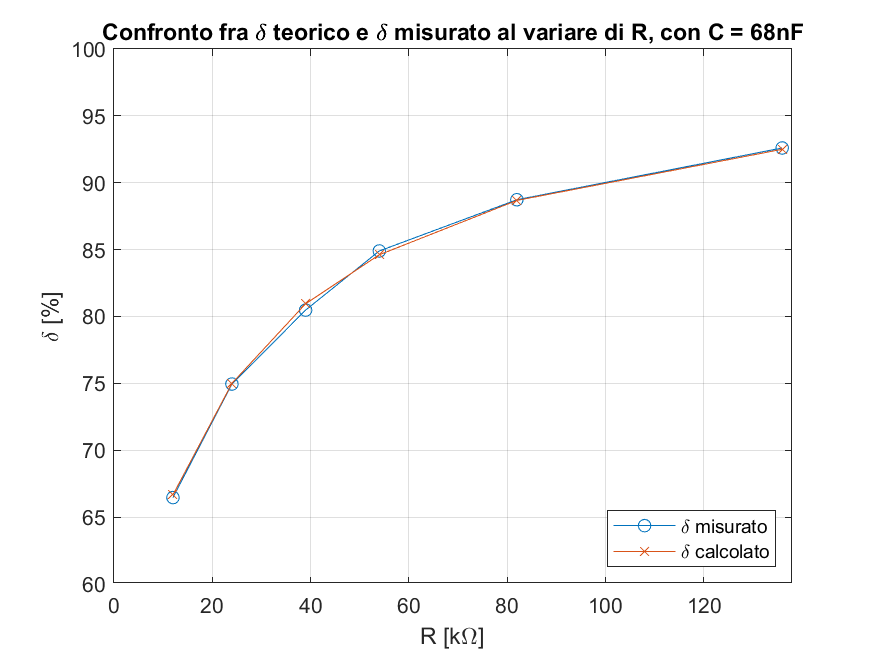
\includegraphics[height=5.8cm]{immagini/graficoDC2}
	\caption{Grafico di T (a sinistra) e $\delta$ (a destra) in funzione di $\mathrm{R_A}$ per $\mathrm{C_1}$ = \SI{68}{n\farad}.}
	\label{figura:graficiC2}
\end{figure}
\begin{figure}[h!]
	\centering
	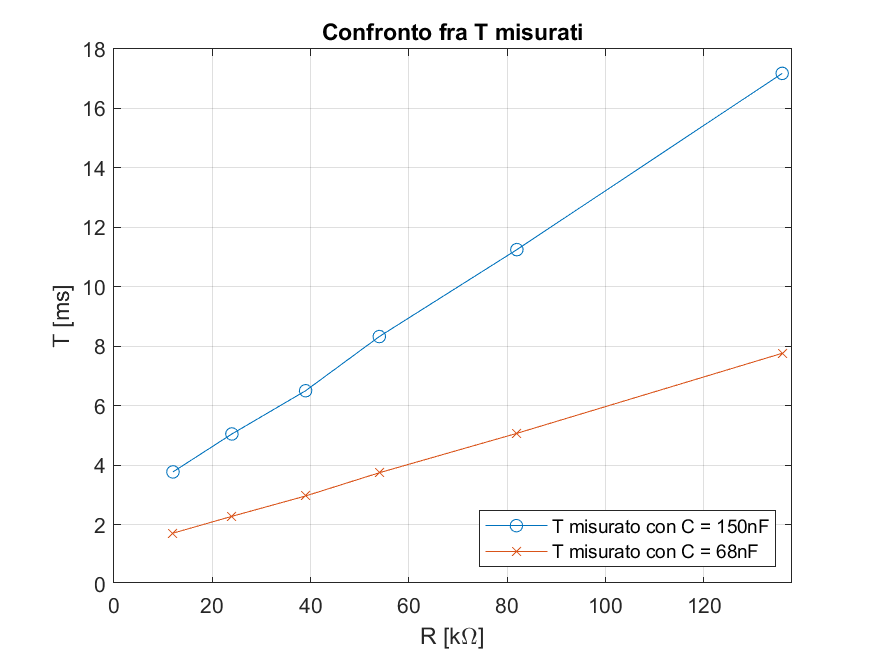
\includegraphics[height=5.8cm]{immagini/graficoConfrontoT}
	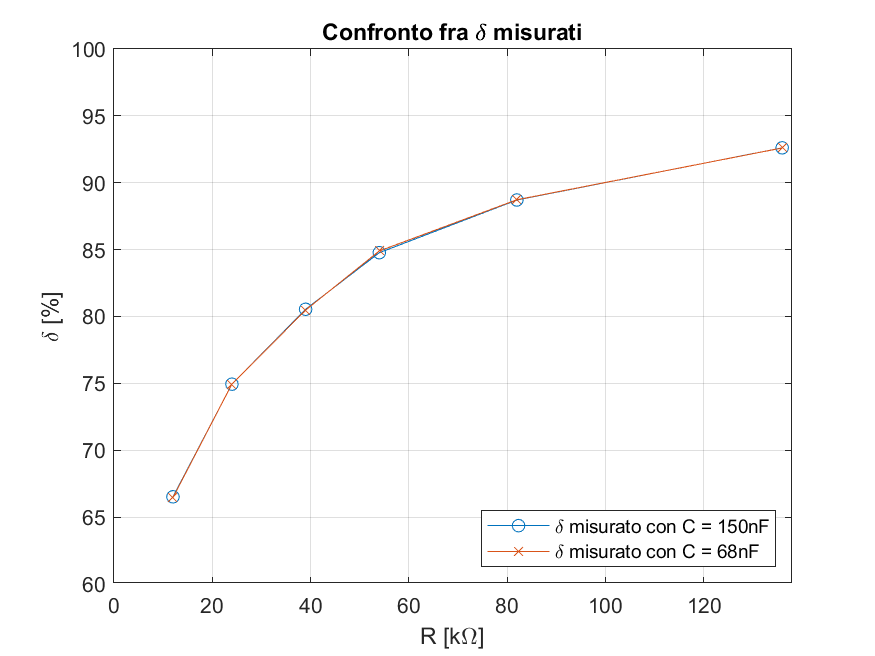
\includegraphics[height=5.8cm]{immagini/graficoConfrontoDC}
	\caption{Grafico di T (a sinistra) e $\delta$ (a destra) in funzione di $\mathrm{R_A}$ per i due valori di capacità.}
	\label{figura:graficiC12}
\end{figure}
\\Dalla figura seguente, invece, vediamo che l'uscita del circuito è effettivamente un'onda quadra (CH2), le cui caratteristiche sono determinate dal ciclo di carica e scarica del condensatore (CH1). I valori dei componenti utilizzati sono quelli mostrati anche nella fotografia di figura \ref{figura:circuito3}.
\begin{figure}[h!]
	\centering
	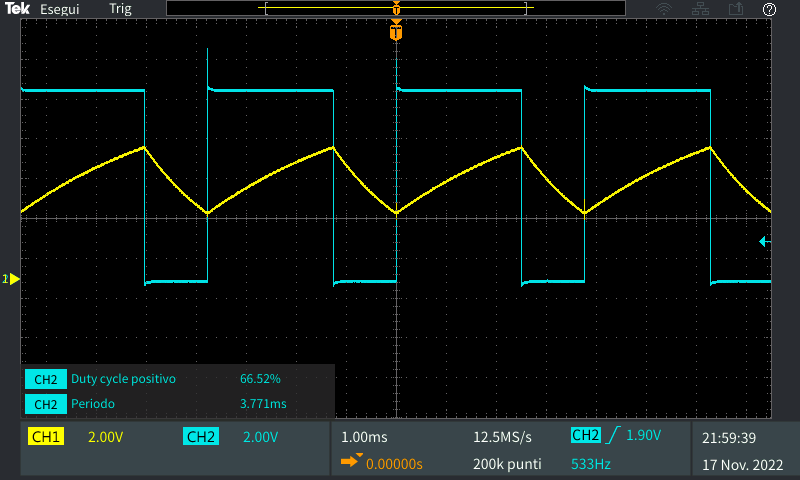
\includegraphics[height=6.5cm]{immagini/TEK00019}
	\caption{Tensione ai capi del condensatore (CH1) e in uscita al circuito (CH2).}
	\label{figura:TEK00019}
\end{figure}
\newpage
\section{Circuito 4: Evoluzione del LM555 in configurazione astabile}
\subsection{Schema del circuito e Funzione di Trasferimento}
Lo svantaggio del circuito appena visto è che siamo vincolati ad avere un duty cycle in uscita limitato fra il 50\% ed il 100\%. Se volessimo ottenere un valore inferiore al 50\%, dobbiamo modificare la rete di carica e scarica del condensatore. Per fare ciò, sostituiamo la resistenza $\mathrm{R_B}$ con un potenziometro, il cui terminale centrale è collegato al condensatore C, mentre gli altri due terminali sono collegati ad un diodo ciascuno, in particolare il terminale di destra è collegato all'anodo, invece quello di sinistra al catodo. I terminali non connessi dei due diodi vengono collegati alla resistenza $\mathrm{R_A}$. Lo schema finale è illustrato in figura \ref{figura:schema4}.
\begin{figure}[h!]
	\centering
	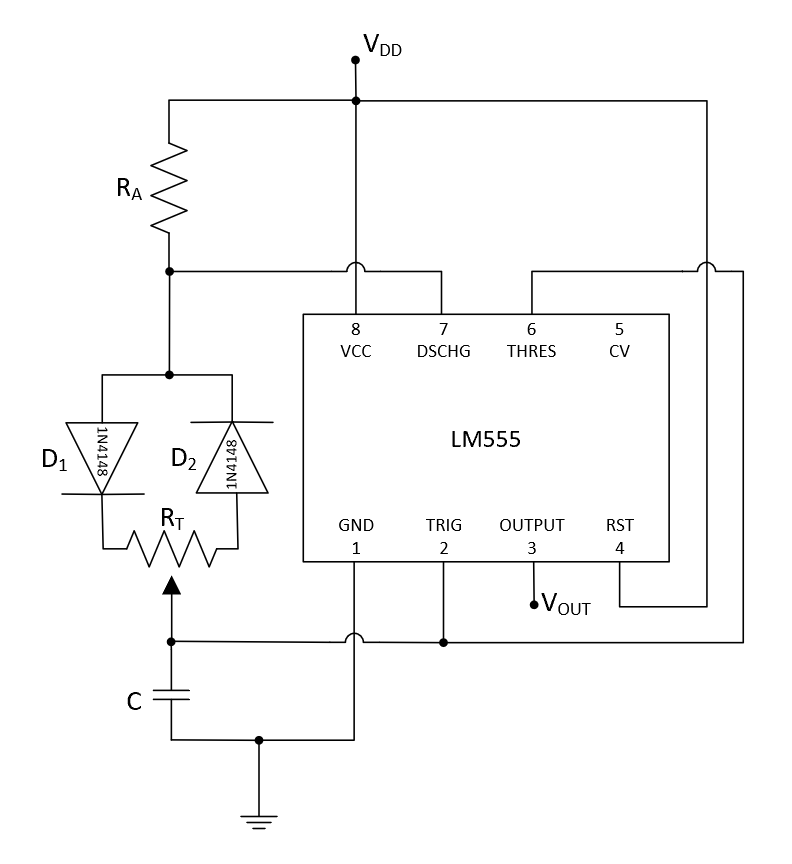
\includegraphics[height=7.5cm]{immagini/schema4}
	\caption{Schema dell'evoluzione del circuito astabile.}
	\label{figura:schema4}
\end{figure}
\\L'intervallo di tempo in cui l'onda quadra rimane alta ($t_1$) e l'intervallo in cui questa rimane bassa ($t_2$) si ricavano dalle leggi di carica e scarica del condensatore e si calcolano come segue:
\\[4pt]\indent$\displaystyle{t_1 = (R_A+R_{T_1})\cdot C_1\cdot \ln2}$
\\[4pt]\indent$\displaystyle{t_2 = (R_{T_2})\cdot C_1\cdot \ln2 = (R_T-R_{T_1})\cdot C_1\cdot \ln2}$
\\[4pt]\indent$\displaystyle{\rightarrow T=t_1+t_2=(R_A+R_{T_1}+R_T-R_{T_1})\cdot C_1\cdot \ln2 = (R_A+R_T)\cdot C_1\cdot \ln2}$
\\[4pt]Il duty cycle dell'onda quadra, $\delta$ si calcola come:
\\[4pt]\indent$\displaystyle{\delta=\frac{t_1}{T}=\frac{(R_A+R_{T_1})\cdot C_1\cdot \ln2}{(R_A+R_T)\cdot C_1\cdot \ln2}=\frac{R_A+R_{T_1}}{R_A+R_T}\simeq\frac{R_{T_1}}{R_T}\mathrm{\; se \;}R_{T}\gg R_A}$
\\[4pt]Dato che il duty cycle è il rapporto fra una porzione di resistenza e la resistenza stessa, e $\displaystyle{R_{T_1} = 0\div R_T}$, il duty cycle può variare tra 0\% e 100\%, quindi questo circuito non è più limitato come il precedente.
\subsection{Analisi e dati sperimentali}
Per realizzare il circuito, di cui si riporta la fotografia in figura \ref{figura:circuito4}, utilizziamo per $\mathrm{R_T}$ un potenziometro che può variare tra \SI{0}{\ohm} e \SI{10}{k\ohm}, quindi per rispettare la condizione $\displaystyle{R_{T}\gg R_A}$ sceglieremo per $\mathrm{R_A}$ una resistenza da \SI{1}{k\ohm} (utilizziamo due resistenze in serie, una da \SI{180}{\ohm} e l'altra da \SI{820}{\ohm}). La capacità $\mathrm{C_2}$ non la utilizziamo, per $\mathrm{C_1}$  invece utilizziamo una capacità da \SI{150}{n\farad}. I valori nominali e misurati delle nuove resistenze sono riportati in tabella \ref{table:res4}.
\begin{figure}[h!]
	\centering
	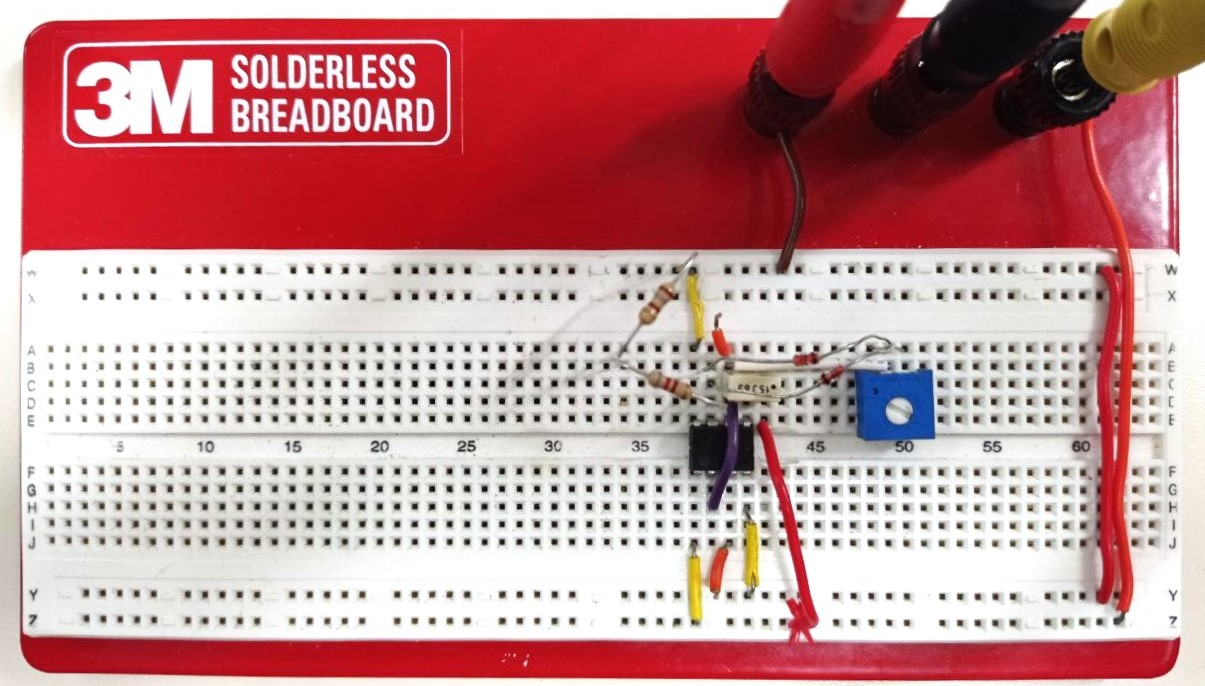
\includegraphics[height=5.7cm]{immagini/circuito4}
	\caption{Fotografia del circuito astabile con potenziometro realizzato in laboratorio.}
	\label{figura:circuito4}
\end{figure}
\begin{table}[h!]
	\centering
	\begin{tabular}{|c|c|c|}
		\cline{2-3} 
		\multicolumn{1}{c|}{} & \textbf{Valore nominale} & \textbf{Valore misurato}\\ 
		\hline
		$\mathbf{R_{A_1}}$ & \SI{180}{\ohm} & \SI{186}{k\ohm} \\ 
		\hline
		$\mathbf{R_{A_2}}$ & \SI{820}{\ohm} & \SI{817}{k\ohm} \\ 
		\hline
		$\mathbf{R_{A}}$ & \SI{1.000}{k\ohm} & \SI{1.003}{k\ohm} \\ 
		\hline
		$\mathbf{R_{T_{min}}}$ & \SI{0}{\ohm} & \SI{0.22}{k\ohm} \\ 
		\hline
		$\mathbf{R_{T_{max}}}$ & \SI{10}{k\ohm} & \SI{10.16}{k\ohm} \\ 
		\hline
	\end{tabular}
	\caption{Misure delle resistenze utilizzate per il circuito.}
	\label{table:res4}
\end{table}
\\ Per analizzare questo circuito, variamo le resistenze $\mathrm{R_{T_1}}$ e $\mathrm{R_{T_2}}$ del potenziometro e misuriamo il duty cycle con l'oscilloscopio. I risultati sono riportati in tabella \ref{table:mis_cto4}.
\begin{table}[h!]
	\centering
	\begin{tabular}{|c|c|c|c|}
		\hline
		$\mathbf{R_{T_1}}$ & $\mathbf{R_{T_2}}$ & $\mathbf\delta$\textbf{ misurato} & $\mathbf\delta$\textbf{ teorico}\\ 
		\hline
		\SI{10.16}{k\ohm} & \SI{0.18}{k\ohm} & 99.42\% & 98.26\% \\ 
		\hline
		\SI{7.33}{k\ohm} & \SI{2.79}{k\ohm} & 74.14\% & 74.43\% \\ 
		\hline
		\SI{5.20}{k\ohm} & \SI{4.96}{k\ohm} & 54.86\% & 51.18\% \\ 
		\hline
		\SI{1.98}{k\ohm} & \SI{8.15}{k\ohm} & 26.60\% & 19.55\% \\ 
		\hline
		\SI{0.22}{k\ohm} & \SI{10.13}{k\ohm} & 9.06\% & 2.13\% \\ 
		\hline
	\end{tabular}
	\caption{Misure e valori teorici del duty cycle al variare della resistenza del potenziometro.}
	\label{table:mis_cto4}
\end{table}
\\Dalla tabella, possiamo vedere che per valori elevati di $\mathrm{R_{T_1}}$, e quindi per valori elevati del duty cycle, i valori teorici e misurati sono abbastanza precisi. Per valori piccoli, invece, le misure hanno un errore elevato. Quest'imprecisione potrebbe essere dovuta al fatto che l'approssimazione del calcolo del duty cycle fatta con la condizione $\displaystyle{R_{T}\gg R_A}$ è troppo forte, dato che le resistenze $\mathrm{R_{T_1}}$ e $\mathrm{R_{A}}$ sono confrontabili. Anche dal grafico seguente, la figura \ref{figura:grafico4} ritroviamo quanto appena detto.
\begin{figure}[h!]
	\centering
	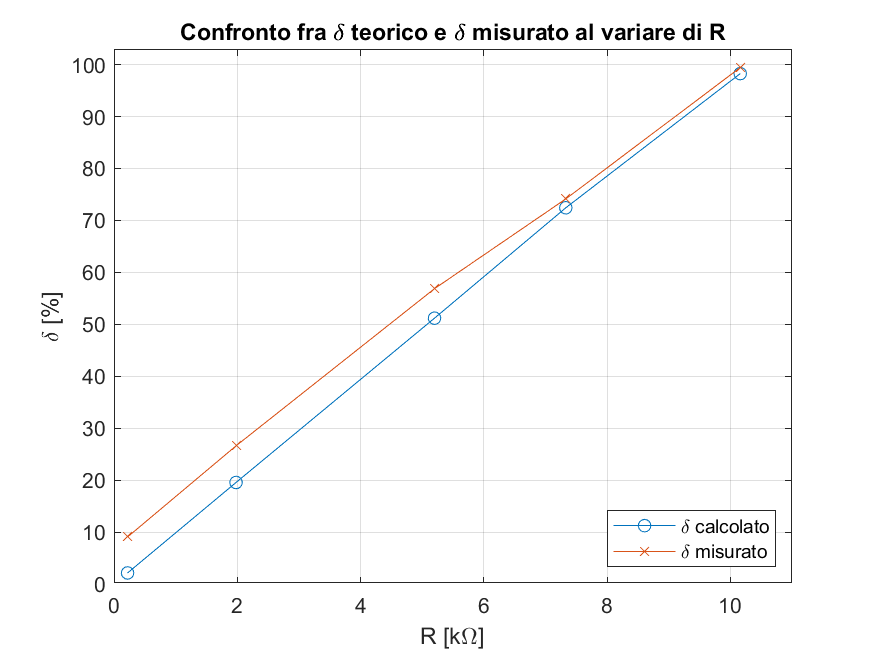
\includegraphics[height=7cm]{immagini/graficomis4}
	\caption{Grafico del confronto fra duty cycle calcolato e misurato.}
	\label{figura:grafico4}
\end{figure}
\\Per verificare che l'origine dell'errore sia l'approssimazione della formula utilizzata per il calcolo del duty cycle, proviamo a tracciare il grafico delle misure in funzione del calcolo del duty cycle senza approssimazione. Il risultato è mostrato nella figura seguente, possiamo vedere che in questo caso le misure sono effettivamente confrontabili con i risultati teorici.
\begin{figure}[h!]
	\centering
	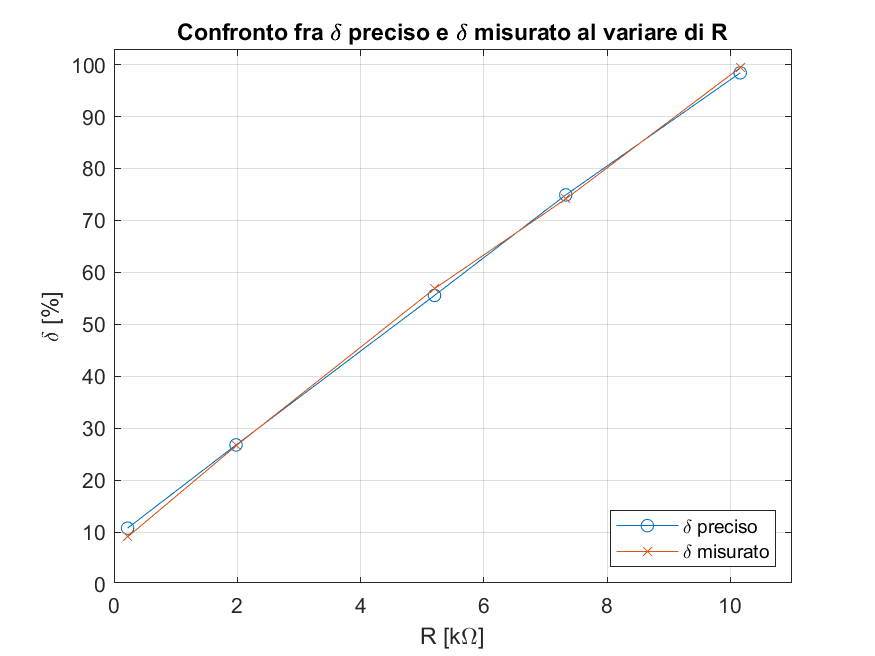
\includegraphics[height=7cm]{immagini/graficomis4_prec}
	\caption{Grafico del confronto fra duty cycle calcolato senza approssimazione e misurato.}
	\label{figura:grafico4_prec}
\end{figure}
\\Il comportamento del circuito è quindi corretto, perciò siamo in grado di ottenere in uscita un'onda quadra con duty cycle variabile da 0\% a 100\%, come si vede anche dai grafici ottenuti dall'oscilloscopio e mostrati in figura \ref{figura:TEK00032e36}.
\begin{figure}[h!]
	\centering
	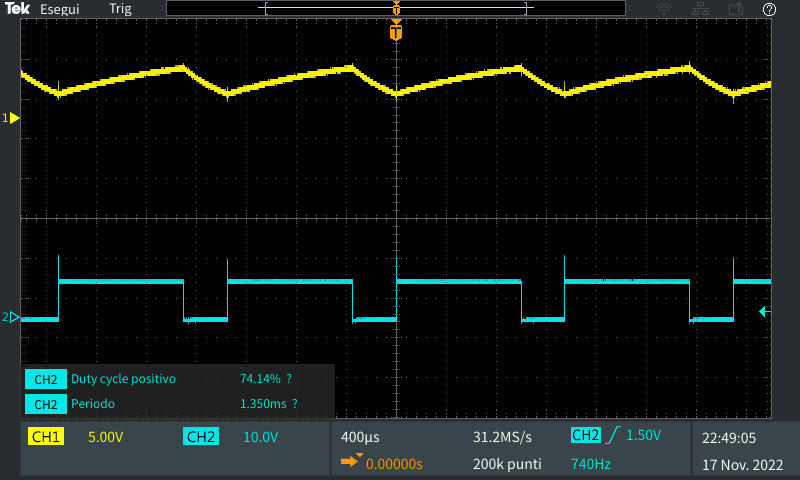
\includegraphics[height=4.6cm]{immagini/TEK00032}
	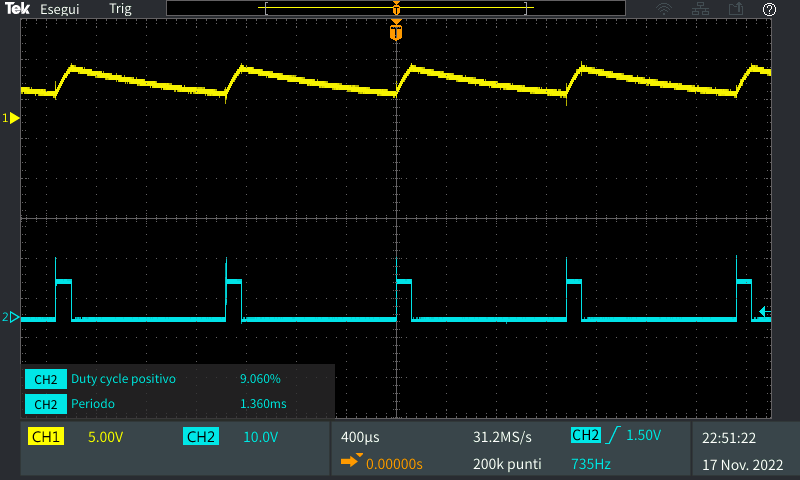
\includegraphics[height=4.6cm]{immagini/TEK00036}
	\caption{Onda quadra in uscita e tensione ai capi del condensatore per due valori di resistenza.}
	\label{figura:TEK00032e36}
\end{figure}

%----------------------------------------------------------------------------------------

\end{document}
